\input{../../template.ltx}
\usepackage{amsmath}
\usepackage{multicol}
\usepackage{graphicx}
\begin{document}

\osuetitle{2}

\section*{Assignment -- Integer Multiplication}
Implement an algorithm for the efficient multiplication of large integers.
\begin{verbatim}
    SYNOPSIS
        intmul
\end{verbatim}

\subsection*{Instructions}
The program takes two hexadecimal integers $A$ and $B$ with an equal number of digits as input, multiplies them and prints the result.
The input is read from \texttt{stdin} and consists of two lines:
the first line is the integer $A$ and the second line is the integer $B$.

Your program must accept any number of digits.
Terminate the program with exit status \verb|EXIT_FAILURE|
if an invalid input is encountered
or if the two integers do not have equal length.

The multiplication of the input values is calculated recursively,
i.e. by the program calling itself:
\begin{enumerate}
\item If $A$ and $B$ both consist of only 1 hexadecimal digit, then multiply them,
write the result to \texttt{stdout} and exit with status \verb|EXIT_SUCCESS|.
\item Otherwise $A$ and $B$ both consist of $n>1$ digits. Split them both into two parts each,
with each part consisting of $n/2$ digits:
\renewcommand{\arraystretch}{1.3}
\[
A:\quad\quad\begin{array}{|c|c|}\hline \quad A_h \quad & \quad A_l \quad \\\hline\end{array}\quad\quad A=A_h\cdot 16^{n/2}+A_l
\]
\[
B:\quad\quad\begin{array}{|c|c|}\hline \quad B_h \quad & \quad B_l \quad \\\hline\end{array}\quad\quad B=B_h\cdot 16^{n/2}+B_l
\]
Terminate the program with exit status \verb|EXIT_FAILURE|
if the number of digits is not even.

\item Using \osuefunc{fork(2)} and \osuefunc{execlp(3)},
recursively execute this program in four child processes,
one for each of the multiplications $A_h\cdot B_h$, $A_h\cdot B_l$, $A_l\cdot B_h$ and  $A_l\cdot B_l$.
Use two unnamed pipes per child
to redirect \osueglvar{stdin} and \osueglvar{stdout}
(see \osuefunc{pipe(2)} and \osuefunc{dup2(3)}).
Write the two values to be multiplied to \osueglvar{stdin} of each child.
Read the respective result from each child's \osueglvar{stdout}.
The four child processes must run simultaneously!

\item Use \osuefunc{wait(2)} or \osuefunc{waitpid(2)}
to read the exit status of the children.
Terminate the program with exit status \verb|EXIT_FAILURE|
if the exit status of any of the two child processes is not \verb|EXIT_SUCCESS|.

\item The result of the multiplication $A\cdot B$ can now be calculated as follows:
\[
A\cdot B=A_h\cdot B_h\cdot 16^n + A_h\cdot B_l\cdot 16^{n/2} + A_l\cdot B_h\cdot 16^{n/2} + A_l\cdot B_l
\]
Find a clever way to write the result of this operation to \texttt{stdout},
even if the numbers are too large for the C data types.
Remember that your program must deal with integers of any size!
Terminate the program with exit status \verb|EXIT_SUCCESS|.

\end{enumerate}

\clearpage
\subsection*{Hints}

\begin{itemize}
\item Think of a way to add the four intermediate results together
one digit at a time while keeping track of the carry.
\item In order to avoid endless recursion\footnote{\url{http://en.wikipedia.org/wiki/Fork\_bomb}},
fork only if the input number is greater than 1.
\item To output error messages and debug messages, always use
\osueglvar{stderr} because \osueglvar{stdout} is redirected in most cases.
\end{itemize}

\subsection*{Bonus exercise, 5 points}
Print the parent and child relations in form of a tree to stdout. Print all children which are forked from the parent.
The tree should be readable at least to a depth of three.
For every node, the intermediate result should be printed.\newline
Depending on how often you call fork the wider the tree becomes. A simple example is shown below.

\begin{figure}[h!]
	\centering
	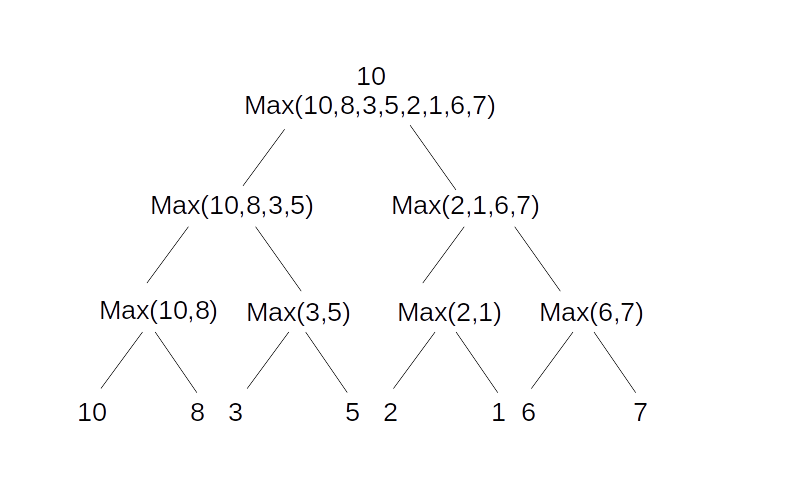
\includegraphics[width=0.5\textwidth]{./../BonusExercise.png}
\end{figure}

\paragraph{Instructions on how to print the tree}
A leaf node should output the substep executed by it on stdout with a terminating newline. Every other node has to do two steps. First, it calculates the intermediate result and outputs this and the executed operation to stdout. Thereafter, symbols that are to represent the branches of the tree are output to stdout. Lastly he parses the output from his children via a pipe. Thereafter, each newline character is removed, the output is lined up and then printed with a terminating newline to stdout.
\subsection*{Examples}
\begin{multicols}{3}
\begin{verbatim}
$ cat 1.txt
3
3
$ ./intmul < 1.txt
9
\end{verbatim}

\begin{verbatim}
$ cat 2.txt
1A
B3
$ ./intmul < 2.txt
122e
\end{verbatim}

\begin{verbatim}
$ cat 3.txt
13A5D87E85412E5F
7812C53B014D5DF8
$ ./intmul < 3.txt
09372e47ae47c3f68e45d1a816906f08
\end{verbatim}
\end{multicols}

\osueguidelinestwo

\end{document}
